\documentclass[11pt,spanish,a4paper]{article}

% Versión 1.er cuat 2021 Víctor Bettachini < vbettachini@unlam.edu.ar >

\usepackage[T1]{fontenc}
\usepackage[utf8]{inputenc}

\usepackage[spanish, es-tabla]{babel}
% \def\spanishoptions{argentina} % Was macht dass?
% \usepackage{babelbib}
% \selectbiblanguage{spanish}
% \addto\shorthandsspanish{\spanishdeactivate{~<>}}


\usepackage{graphicx}
\graphicspath{{./figuras/}{../LaTeX/}{../figurasLaTeX/}}
% \usepackage{float}

\usepackage[arrowdel]{physics}
\newcommand{\pvec}[1]{\vec{#1}\mkern2mu\vphantom{#1}}
% \usepackage{units}
\usepackage[separate-uncertainty= true, multi-part-units= single, range-units= single, range-phrase= {~a~}, locale= FR]{siunitx}
\usepackage{isotope} % $\isotope[A][Z]{X}\to\isotope[A-4][Z-2]{Y}+\isotope[4][2]{\alpha}

\usepackage{tasks}
\usepackage[inline]{enumitem}
% \usepackage{enumerate}

\usepackage{hyperref}

% \usepackage{amsmath}
% \usepackage{amstext}
% \usepackage{amssymb}

\usepackage{tikz}
\usepackage{tikz-3dplot}
\usepackage{tikz-dimline}
\usetikzlibrary{calc}
% \usetikzlibrary{math}
\usetikzlibrary{arrows.meta}
\usetikzlibrary{snakes}
\usetikzlibrary{decorations}
\usetikzlibrary{decorations.pathmorphing}
\usetikzlibrary{patterns}

\usepackage[hmargin=1cm,vmargin=3cm, top= 0.75cm,nohead]{geometry}

\usepackage{lastpage}
\usepackage{fancyhdr}
\pagestyle{fancyplain}
\fancyhf{}
\setlength\headheight{28.7pt} 
\fancyhead[LE, LO]{\textbf{Mecánica Analítica Computacional} }
% \fancyhead[LE, LO]{\textbf{Mecánica General} }
\fancyhead[RE, RO]{\href{https://ingenieria.unlam.edu.ar/}{$\vcenter{\hbox{
\includegraphics[height=1cm]{ambos.pdf}}}$}}
\fancyfoot{\href{https://creativecommons.org/licenses/by-nc-sa/4.0/deed.es_ES}{$\vcenter{\hbox{
\includegraphics[height=0.4cm]{by-nc-sa_80x15.pdf}}}$} \href{https://ingenieria.unlam.edu.ar/}{DIIT - UNLaM}}
\fancyfoot[C]{ {\tiny Actualizado al \today} }
\fancyfoot[RO, LE]{Pág. \thepage/\pageref{LastPage}}
\renewcommand{\headrulewidth}{0pt}
\renewcommand{\footrulewidth}{0pt}


\begin{document}
\begin{center}
  \textsc{\large Mecánica general}\\
  \textsc{\large Movimiento rotatorio | Momento angular | Torque}
\end{center}

%De poder resolver estos problemas en forma autónoma puede asumir que adquirió los conocimientos mínimos sobre los temas abordados.
%No dude en consultar a docentes y compañeros si no puede terminarlos.
% Los problemas marcados con * son opcionales.
\begin{enumerate}


\section*{Movimiento rotatorio}

\item
\begin{minipage}[t][6cm]{0.65\textwidth}
% \textbf{FCEyN g01e03 | MIT2_003SCF11Kinematic.pdf}
Un frisbee tiene su masa $M$ distribuida en forma uniforme en su radio $R$.
Mientras gira manteniendo su horizontalidad una araña que estaba originalmente en su centro camina en dirección radial a velocidad constante $v_a$.
\begin{enumerate}[label=\alph*)]
	\item Escribir la expresión velocidad y aceleración de la araña consideradas desde un sistema de coordenadas fijas al suelo.
	\item ¿Cuál es la $\omega$ del frisbee respecto a la original cuando la araña esté a una distancia $d$ de su centro?
	\item ¿Qué torque debiera ejercerse al frisbee si se quisiera que su $\omega$ fuera constante?
	¿Qué fuerza de \emph{coriolis} siente la araña en tal caso?
\end{enumerate}
\end{minipage}
\begin{minipage}[c][0cm][t]{0.3\textwidth}
	\includegraphics[width=\textwidth]{\detokenize{arañaFrisbee.png}}
\end{minipage}


\item
\begin{minipage}[t][9cm]{0.65\textwidth}
% \textbf{MIT2_003SCF11_pset2.pdf ej5}
Un bloque de masa $M_b$ está restringido a un movimiento horizontal por rodillos.
Designemos la aceleración horizontal del bloque en un marco de referencia inercial $O_{xyz}$ como $\vec{a}_{A/O} = \ddot{x} \hat{x}$ que asumiremos conocida.
El punto $A$ está fijo al bloque.
Una barra sin masa rota en torno al punto $A$ con una $\dot{\theta}$ constante.
Una masa puntual $m$ está conectada al final de la barra en el punto $B$.

Este problema presenta uno de los problemas más comunes en ingeniería mecánica - el rotor mal balanceado.
Pueden ver una ilustración extrema de este efecto en este video: \url{https://youtu.be/R2hO--TIjjA}.

\begin{enumerate}[label=\alph*)]
	\item Encuentre una expresión para la aceleración de la masa $m$ en el sistema de referencia inercial $O_{xyz}$.
	Esto es encontrar $\vec{a}_{B/O}$.
	Exprese el resultado en términos de las componentes $x$ e $y$ en el sistema $O_{xyz}$.
	Recuerde incluir la contribución de $\vec{a}_{A/O}= \ddot{x} \hat{x}$ en su respuesta.
	\item ¿Cuál es la magnitud y dirección de la fuerza que la barra aplica a la masa $m$?
	¿Cuál es la fuerza y dirección de la misma que la barra hace sobre el punto de pivot A?
\end{enumerate}
\end{minipage}
\begin{minipage}[c][0cm][t]{0.3\textwidth}
	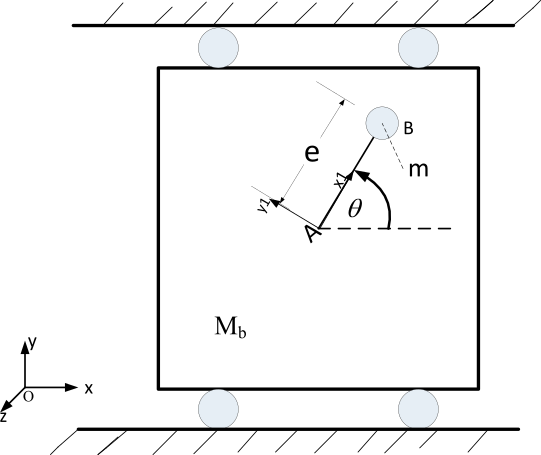
\includegraphics[width=\textwidth]{MIT2_003SCF11_pset2_figure5}
\end{minipage}
Pregunta conceptual:
La posición del centro de masa del sistema que conforman el bloque y la masa en rotación puede calcularse en función de la posición de la barra a medida que esta rota.
Cuando se lo analiza desde un sistema de referencia inercial externo al bloque, este centro de masa: 
\begin{enumerate}[label=\alph*),itemjoin={,\quad}]
	\item se mueve a la izquierda cuando la bola está en la mitad izquierda del recorrido circular,
	\item se mueve a la derecha cuando la bola está en la mitad izquierda del recorrido circular,
	\item o no se mueve ni a izquierda ni a derecha.
\end{enumerate}



\section*{Momento angular | Torque}

\item
\begin{minipage}[t][6.5cm]{0.65\textwidth}
% \textbf{MIT2_003SCF11_pset3_e01}
Un satélite cilíndrico rota en torno a su eje de simetría con $\Omega= \SI{0,05}{\per\second}$.
Dos instrumentos científicos $P$ están originalmente a $R=\SI{1,2}{\metre}$ de tal eje, pero conectados a barras radiales extensibles.
La posterior extensión de su longitud $l$ se produce a una tasa constante hasta alcanzar los \SI{3}{\metre}.
Durante el procedimiento opera un mecanismo interno que mantiene constante la velocidad de rotación del satélite.
La máxima aceleración total que estos instrumentos pueden ser sometidos es \SI{0,011}{\metre\per\second\squared}.
Determinar la máxima tasa de extensión de las barras.

Pregunta conceptual:
¿Cambia el momento angular total del satélite como resultado de la extensión de las barras que soportan los instrumentos?
Asumamos que el momento angular se calcula con respecto al centro de masa del satélite.
\end{minipage}
\begin{minipage}[c][1cm][t]{0.3\textwidth}
	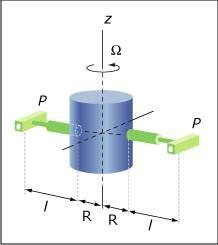
\includegraphics[width=\textwidth]{MIT2_003SCF11_pset2_e01}
\end{minipage}




%\item
%\begin{minipage}[t][5cm]{0.55\textwidth}
%% \textbf{MIT2_003SCF11_pset3_e03}
%Una mujer de \SI{75}{\kilo\gram} salta del carro $A$ con una velocidad horizontal de \SI{3}{\metre\per\second} medida en relación con el carro $A$.
%Los carros $A$ y $B$ tienen la misma masa de \SI{50}{\kilo\gram} y están originalmente en reposo.
%\begin{enumerate}[label=\alph*)]
%	\item Determina la velocidad del carro $A$ justo después de que ella salte.
%	\item Si luego aterriza en el carro $B$ y aparece detenido relativo al carro $B$, determine la velocidad del carro $B$ justo después de que aterrice en ella.
%\end{enumerate}
%\end{minipage}
%\begin{minipage}[c][0cm][t]{0.4\textwidth}
%	\includegraphics[width=\textwidth]{MIT2_003SCF11_pset3_e03}
%\end{minipage}
%Pregunta conceptual:
%Mientras la mujer está en el aire, la velocidad relativa entre ella y el carro $A$ es de \SI{3}{\metre\per\second}.
%Después de que aterrice en el segundo carro, ¿cómo cambiará la velocidad relativa entre ella y el primer carro?
%\begin{enumerate}[label=\alph*),itemjoin={,\quad}]
%	\item Aumentará.
%	\item Disminuirá.
%	\item No sé qué principio aplicar.
%\end{enumerate}


\item
\begin{minipage}[t][4.5cm]{0.5\textwidth}
% \textbf{MIT2_003SCF11_pset3_e03}
Un brazo de longitud $\SI{4}{\metre}$ sin masa gira sobre un eje vertical.
En el borde exterior del mismo hay un carro que para este problema consideraremos como una partícula puntual de masa $\SI{100}{\kilo\gram}$.
El brazo en el eje de rotación aplica el torque, $\vec{M}(t)= \SI{30}{\newton\metre\per\second\squared} \times t^2 \hat{z}$.
Además una fuerza externa $\vec{F}(t)= \SI{15}{\newton\per\second} \times t \hat{\varphi}$ empuja el carro en la dirección tangencial.
La fuerza y el torque se aplican a partir de $t=0$.
\end{minipage}
\begin{minipage}[c][2cm][t]{0.45\textwidth}
	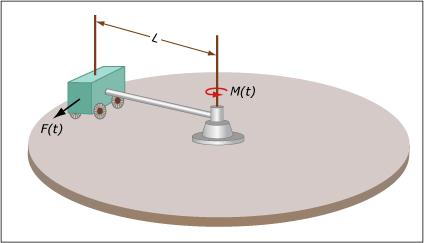
\includegraphics[width=\textwidth]{MIT2_003SCF11_pset3_e05}
\end{minipage}

\begin{enumerate}[label=\alph*)]
	\item Calcule el momento angular del carro con respecto al punto del eje de rotación donde la varilla se une al pivote.
	\item A $t= \SI{5}{\second}$ las fuerzas motrices externas y los torques se apagan, dejando el brazo y carro con una velocidad de rotación constante.
	Calcule el momento lineal del carro $\vec{p}$ para $t>\SI{5}{\second}$.
	\item Calcule la derivada temporal de $\vec{p}$ con respecto al marco inercial de $O_{xyz}$ en $t> \SI{5}{\second}$.
	Explique el significado físico de lo obtenido.
\end{enumerate}

Pregunta conceptual:
¿Qué espera produzca $\dv{\vec{p}}{t}$?
\begin{enumerate*}[label=\alph*),itemjoin={,\quad}]
	\item $\SI{0}{\newton}$
	\item $M g$
	\item Fuerza tangencial
	\item Fuerza radial
\end{enumerate*}


\end{enumerate}
\end{document}
